\documentclass[landscape]{article}

\usepackage[left=1cm,top=2cm,right=1cm,bottom=1cm]{geometry}

\usepackage{tikz}
\usetikzlibrary{calendar}


\pagestyle{empty}

\begin{document}

	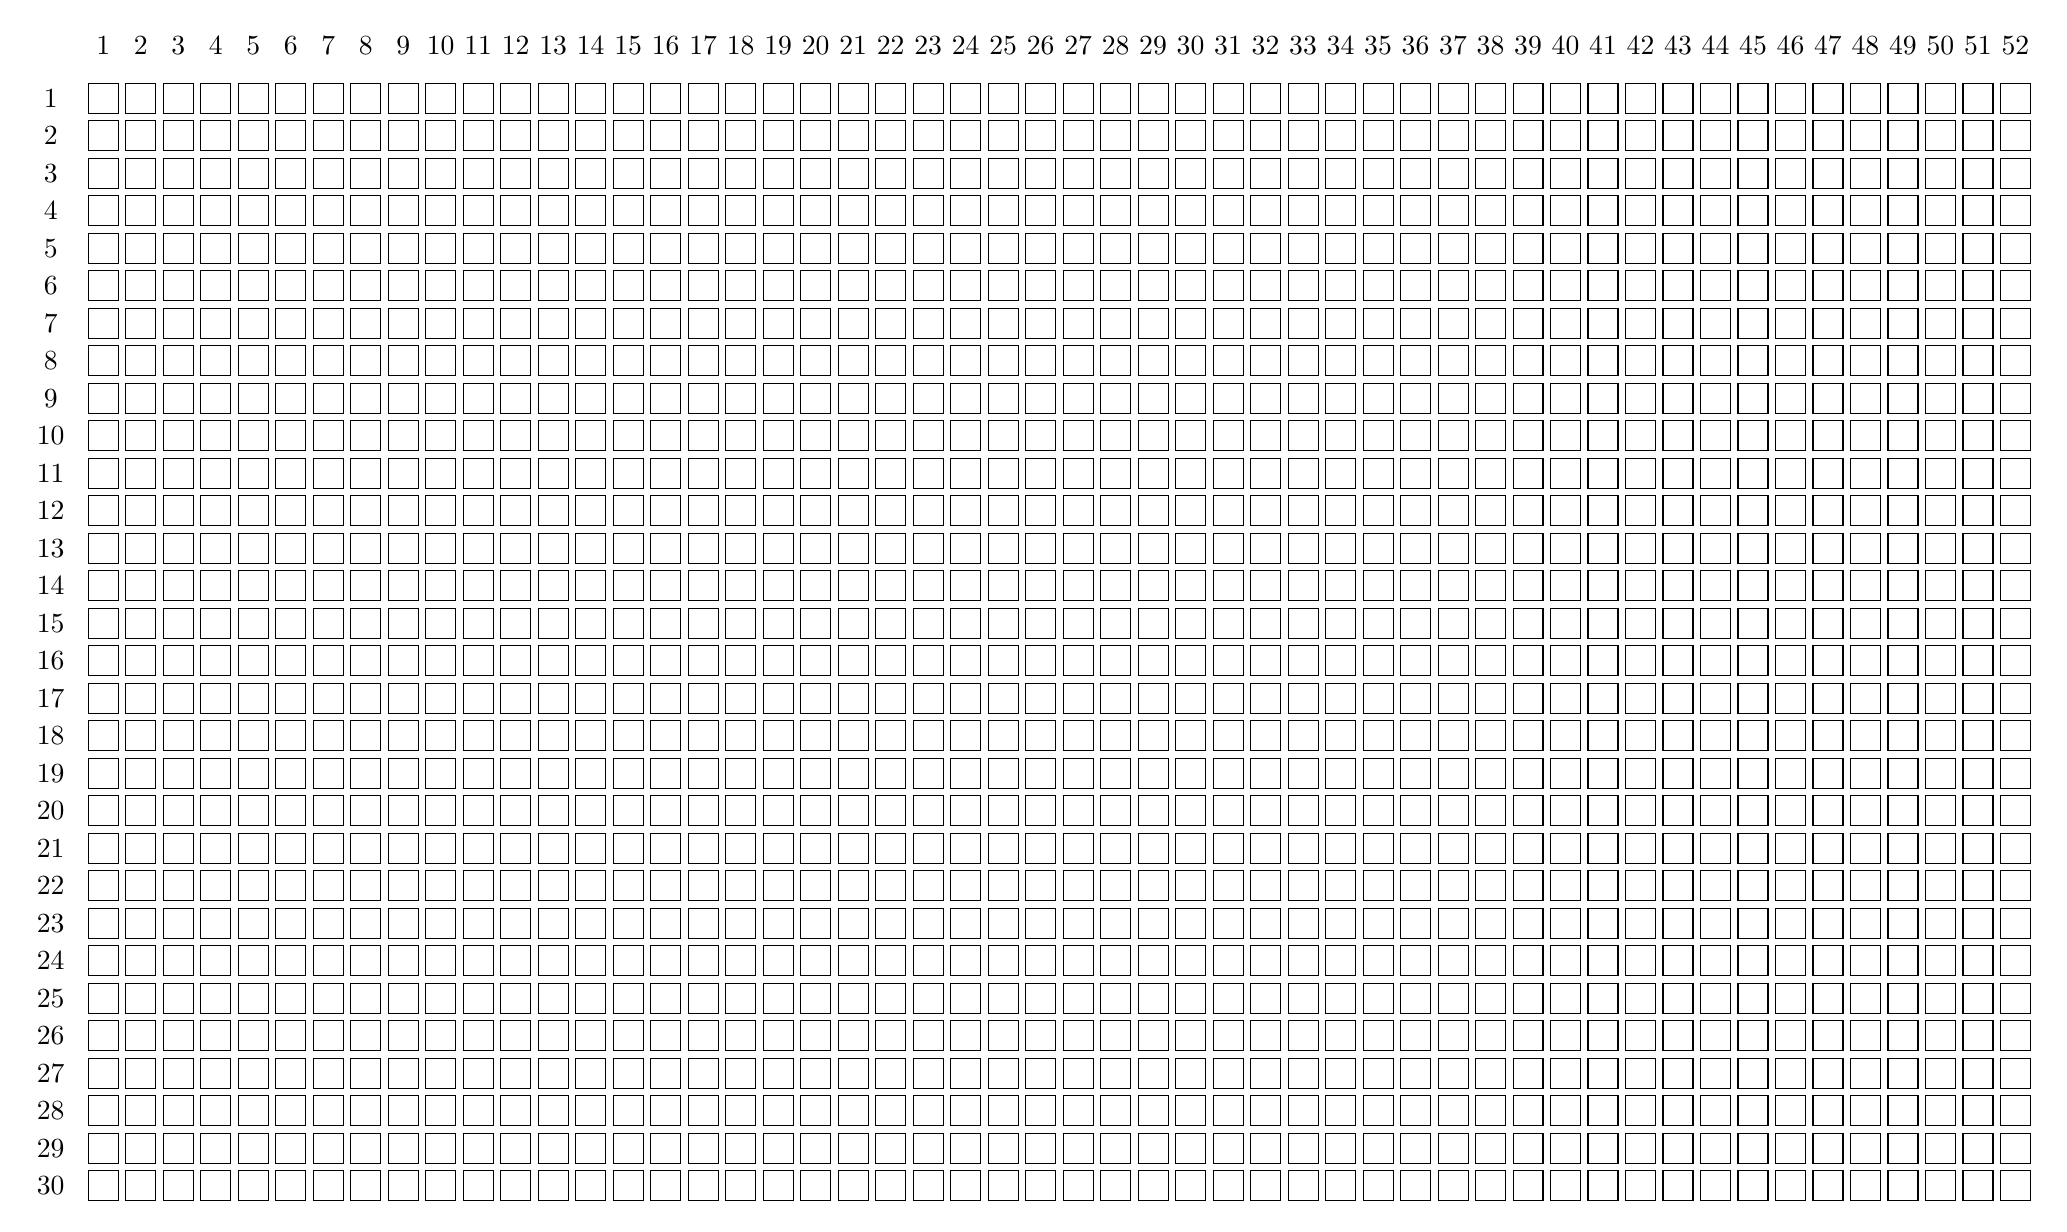
\begin{tikzpicture}
		\def\scale{2.1}
		\def\width{.8}
		\foreach \c in {1,2,...,52}
		{
			\node[] () at (\c/\scale + \width/\scale/2, 0) {$\c$};
		}		
		\foreach \r in {1,2,...,30}
		{
			\node[] () at (0, -\r/\scale - \width/\scale/2) {$\r$};
			\foreach \c in {1,2,...,52}
			{
				\draw[] 
				(\c/\scale, -\r/\scale) 
				rectangle 
				(\c/\scale + \width/\scale, -\r/\scale - \width/\scale);
			}	
		}
	\end{tikzpicture}
	\newpage
	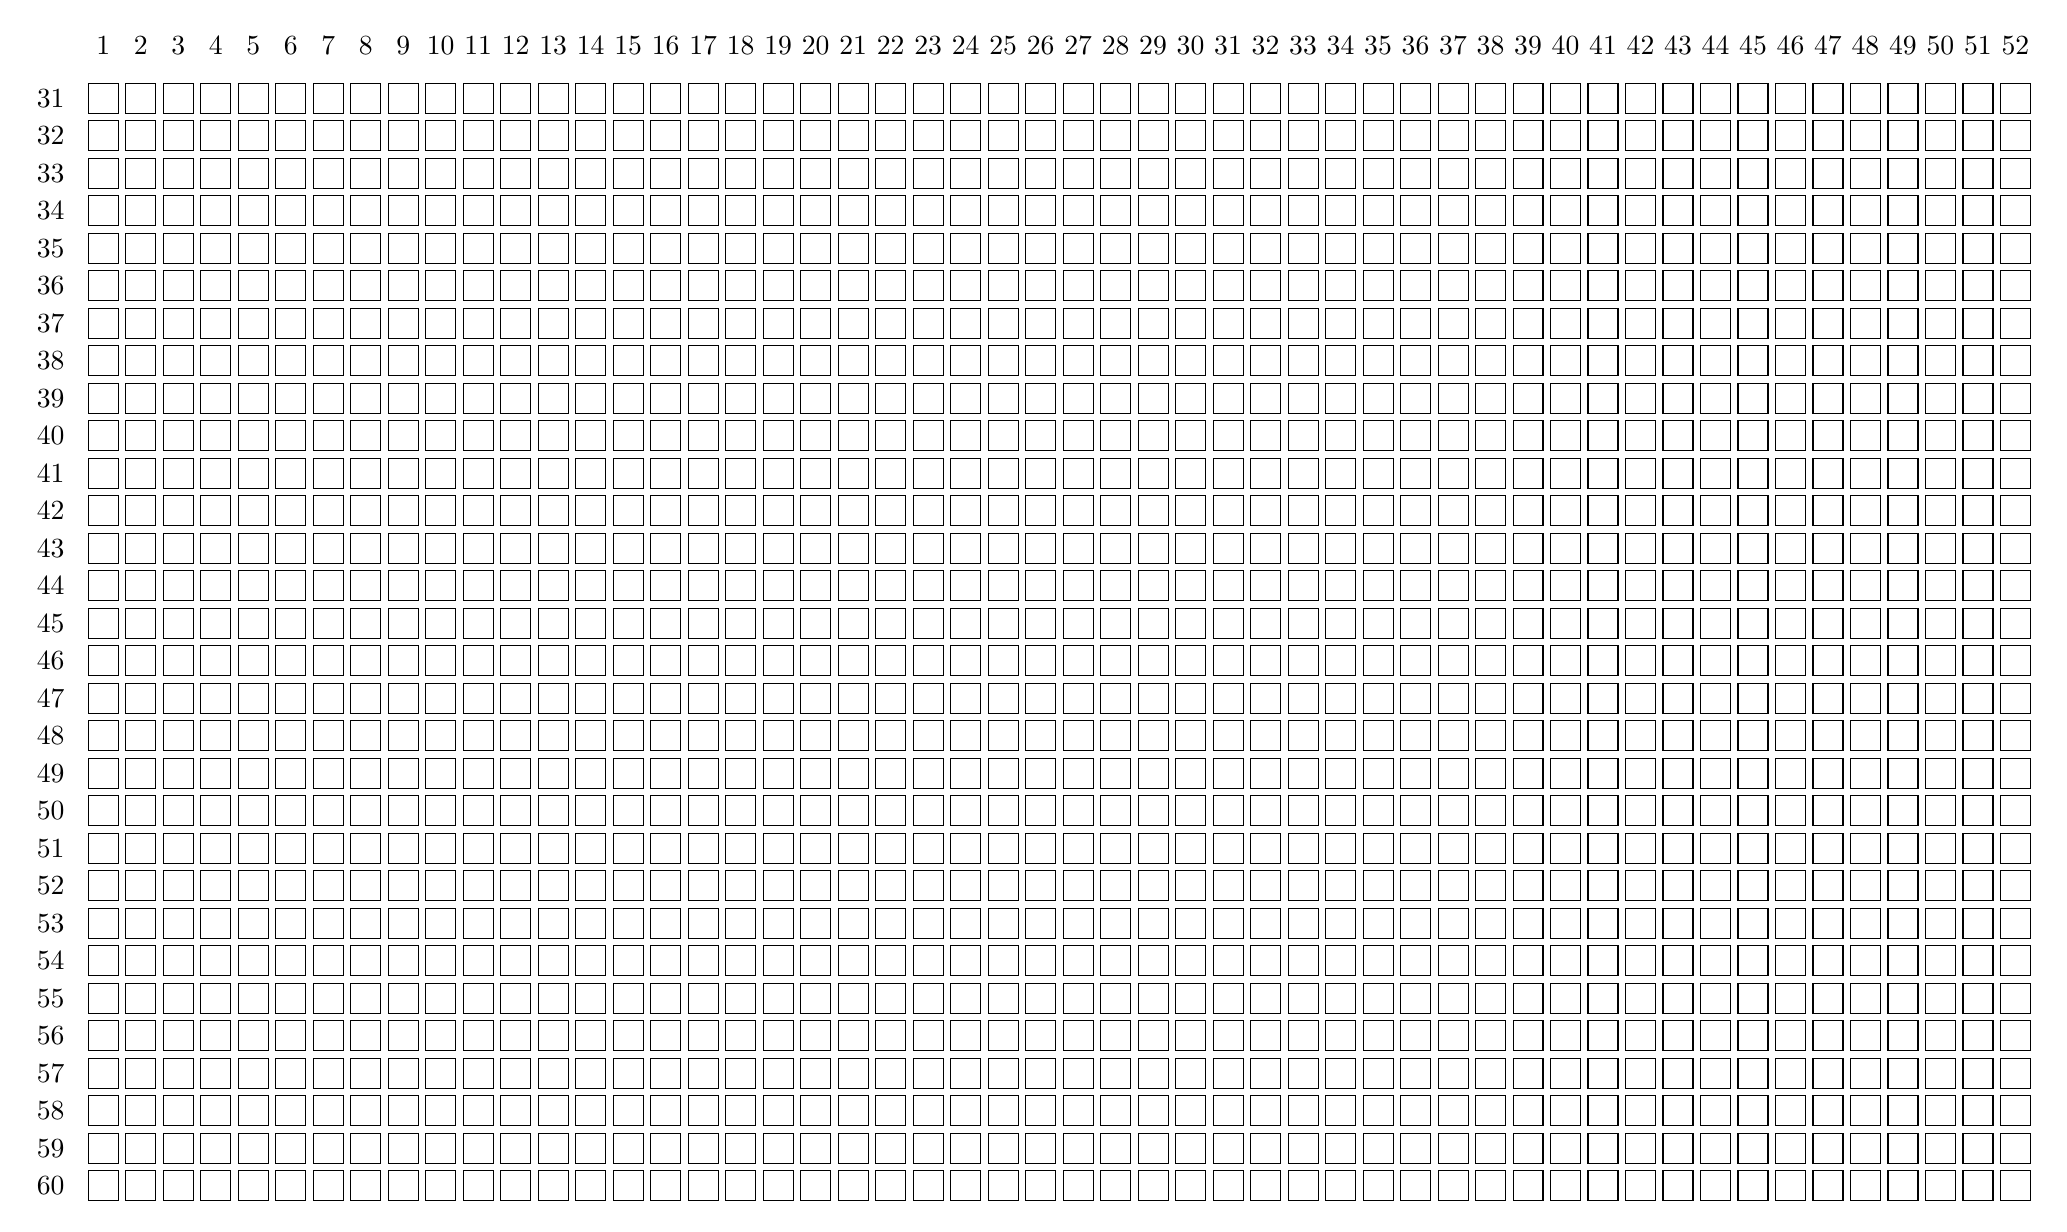
\begin{tikzpicture}
		\def\scale{2.1}
		\def\width{.8}
		\foreach \c in {1,2,...,52}
		{
			\node[] () at (\c/\scale + \width/\scale/2, -30/\scale) {$\c$};
		}		
		\foreach \r in {31,32,...,60}
		{
			\node[] () at (0, -\r/\scale - \width/\scale/2) {$\r$};
			\foreach \c in {1,2,...,52}
			{
				\draw[] 
				(\c/\scale, -\r/\scale) 
				rectangle 
				(\c/\scale + \width/\scale, -\r/\scale - \width/\scale);
			}	
		}
	\end{tikzpicture}
	\newpage
	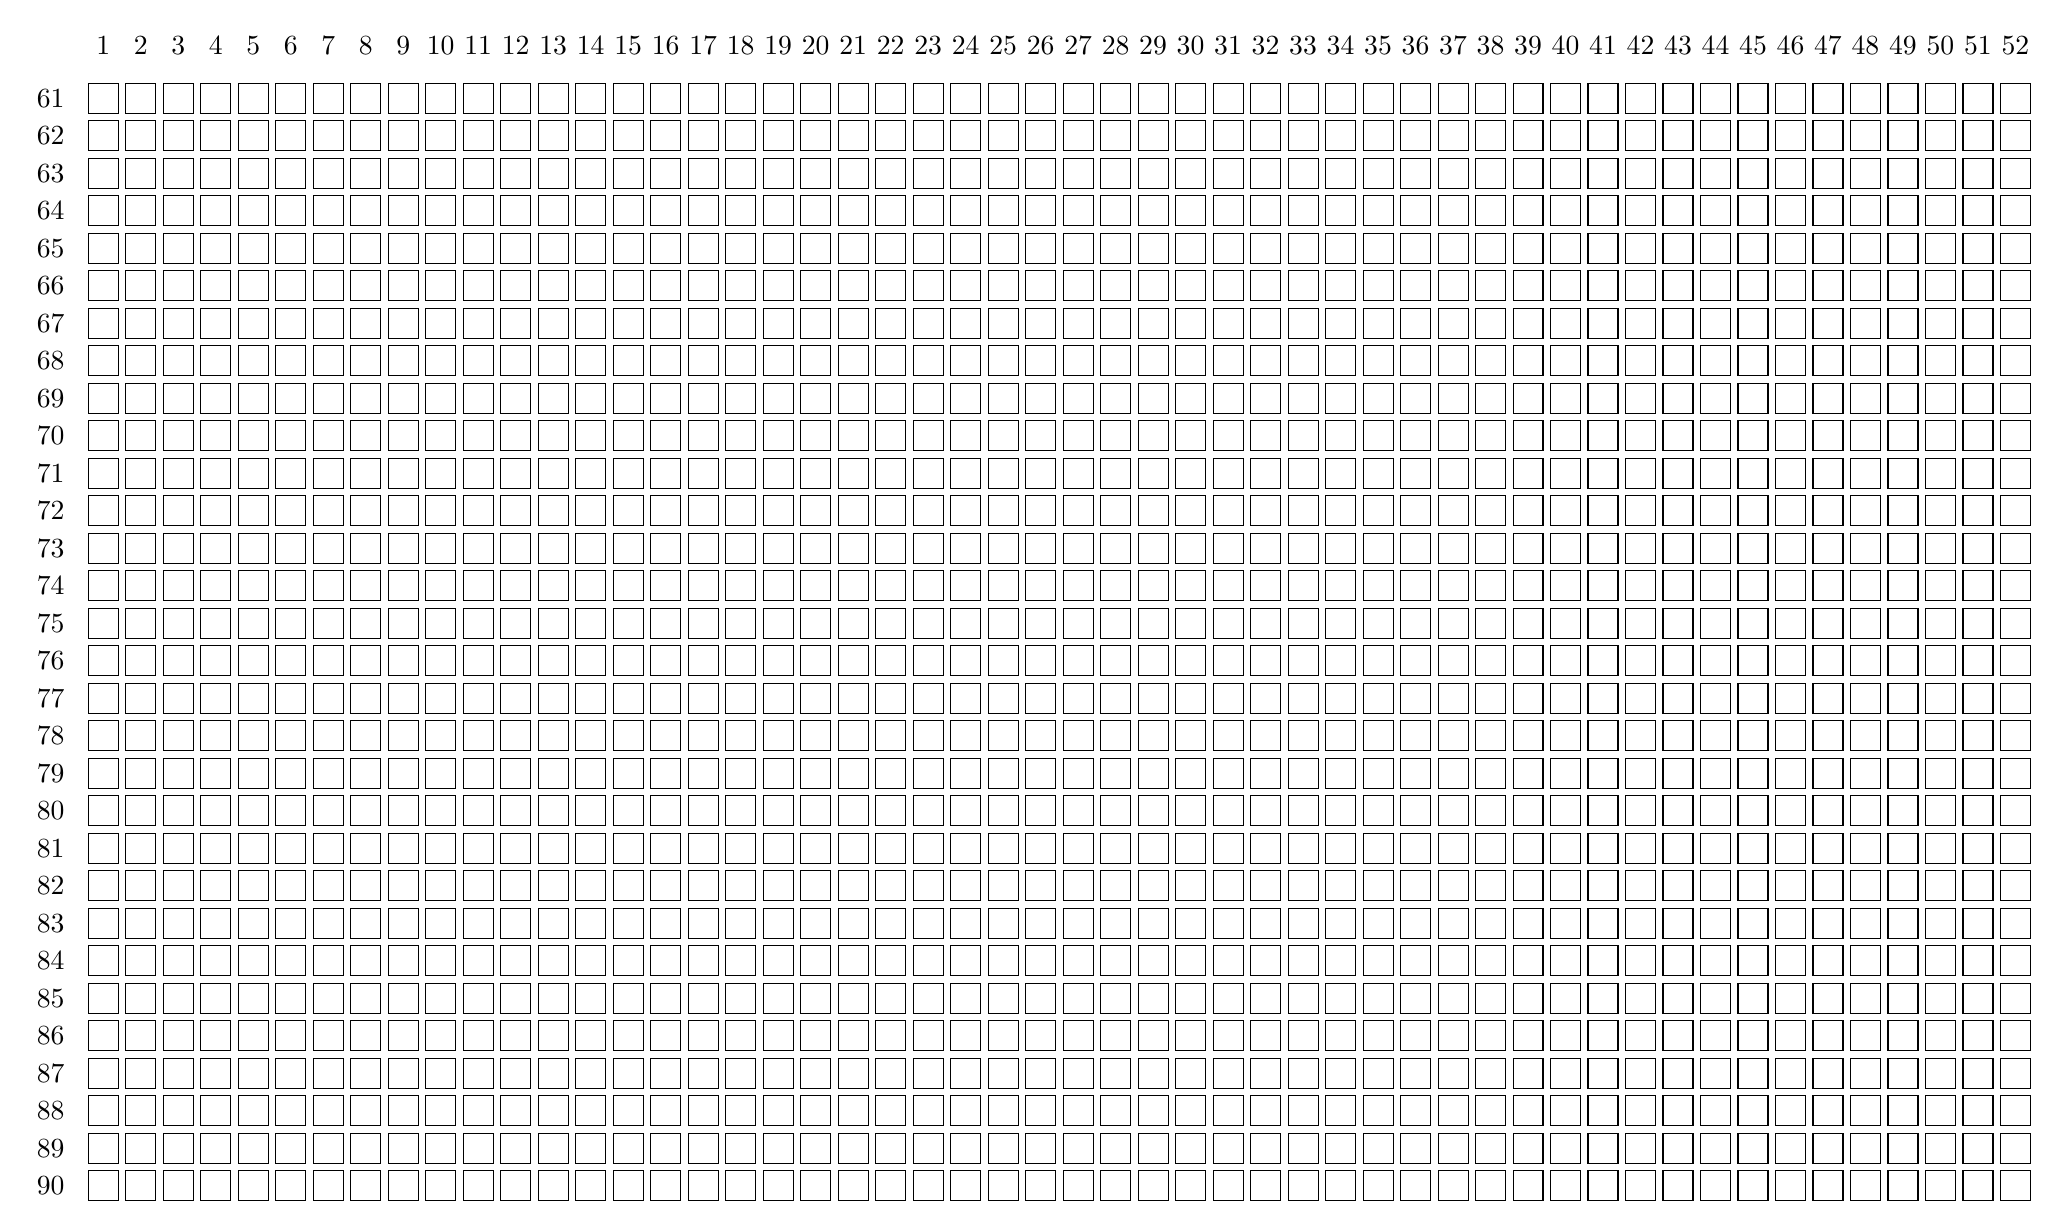
\begin{tikzpicture}
		\def\scale{2.1}
		\def\width{.8}
		\foreach \c in {1,2,...,52}
		{
			\node[] () at (\c/\scale + \width/\scale/2, -60/\scale) {$\c$};
		}		
		\foreach \r in {61,62,...,90}
		{
			\node[] () at (0, -\r/\scale - \width/\scale/2) {$\r$};
			\foreach \c in {1,2,...,52}
			{
				\draw[] 
				(\c/\scale, -\r/\scale) 
				rectangle 
				(\c/\scale + \width/\scale, -\r/\scale - \width/\scale);
			}	
		}
	\end{tikzpicture}

\end{document}